\documentclass[12pt]{report}
\usepackage[utf8]{inputenc}
\usepackage{datetime}

% graphicx
\usepackage{graphicx}
\graphicspath{{images/}}

% biblatex
\usepackage[square,numbers]{natbib}
\bibliographystyle{unsrtnat}

\usepackage[nottoc]{tocbibind}

\title{
    {Deep Q-learning in Grid Worlds}
}
\author{Mihnea Ungureanu}

\begin{document}

\maketitle

\chapter*{Abstract}
Over the relatively recent years, \textbf{reinforcement learning (RL)} has gained immense popularity.
A multitude of interesting results in this field focuses on agents learning in simple, game-like, 2D grid-based environments.

In this paper, we focus on one particular technique in RL -- Q-learning -- and its applications in grid-based, game-like environments.

Classic Q-learning was an early breaktrhough in RL.
We document its evolution and build a survey of improvements over the original.
These techniques are used in practice and have good results in certain areas, such as playing Atari games.
We give examples of succesful applications and explain why Q-learning played a key role.
Finally, we look at advantages and disadvantages over other techniques in RL.

\tableofcontents

\chapter{Short Introduction to RL}
\section{What is Reinforcement Learning?}

\textbf{Reinforcement learning (RL)} is a subset of machine learning that has its origins in computer science and artificial intelligence techniques established in the 1950s.
RL is unique within machine learning as it is focused on goal-directed learning from agent-environment interaction\cite{rlai}.
Simply put, agents learn from environment interactions and gain experience.
They use this experience to optimize their behaviour to achieve problem-defined goals.
This nature-inspired approach captures a broader definition of intelligence (in a human sense) than systems that reason about the world using a finite set of logical rules (i.e., knowledge-based systems).
Like most other subfields of ML, RL is a class of problems as well as a class of solutions to those problems\cite{rlai}.

Advances in the field of deep learning (a broad family of methods based on artificial neural networks\cite{wiki:Deep_learning}) that could enhance the classical algorithms used in RL led to the expansion of the field -- marking the birth of \textbf{deep reinforcement learning (deep RL)}.
Deep RL has surged recently after a series of new algorithms and succesful applications were released. In the following paragraphs, we will summarize some of the most significant results.

\textbf{AlphaGo} (2015)\cite{ago} managed superhuman performance in the game of Go, beating 18-time world champion Lee Sedol.
In late 2017, the AlphaGo family was expanded to contain AlphaGo Zero and AlphaZero\cite{azero}.
Both systems have managed to surpass all their predecessors in game performance, as well as training efficiency \cite{wiki:AlphaGo} (a lot less training time was required to beat the record).
The key difference was that their training was done with absolutely no expert knowledge for either system (hence the ``zero'').
Instead, everything was learned by self-play \cite{azero}.

\textit{Mnih et al.}'s \textbf{DQN}\cite{atari-dqn} (2013) managed human-level performance at seven classic Atari games.
Following the success of DQN, the community worked to improve the standard algorithms.
\textbf{Rainbow DQN} (2017)\cite{rainbow-dqn} is the culmination of that work.
The authors succesfully combined multiple high-quality improvement methods over the original DQN.
The resulting algorithm set a new record on the Atari benchmark.

\textbf{OpenAI Five}\cite{openai-dota} (2018) produced a bot that managed to beat top professional Dota 2 players in international championships.

Despite most of the above list being focused on achievements in video games, RL has been applied to other problems including robot control, elevator scheduling, telecommunications\cite{wiki:Reinforcement_learning}.

\section{Fundamental Components}

First of all, we present the agent-environment feedback loop, as it is crucial to understand the dynamic. An agent acts upon the environment, which reacts according to its set of governing rules.
\begin{enumerate}
    \item The agent receives a reward for this action. This (immediate) reward signal is problem-defined and quantifies the agent’s goal. (see the Reward Hypothesis).
    \item The environment reaction sends the agent into the next state.
    \item The agent perceives and needs to decide on its next action.
\end{enumerate}

\begin{figure}[h]
    \caption{The interaction loop. (Partial reproduction from \cite{rlai}, 3.2)}
    \centering
    \vspace*{0.5cm}
    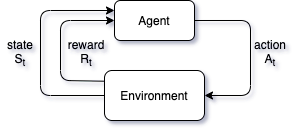
\includegraphics[width=0.5\textwidth]{agent-env-fig}
\end{figure}

\subsection{State and Policy}

We use the concept of \textbf{state}. The state most often refers to the internal state of the agent. Although, in some contexts, we can use it to mean the environment state.
A state contains relevant information from the environment at a given time-step.
A key point in RL is that a well-engineered (agent) state captures all the relevant information and removes the need of explicitly memorizing state history.
This is mathematically by described the \textbf{Markov property}\cite{silver-lectures}, a fundamental property of the mathematical framework underpinning RL -- Markov decision processes (MDPs).

A \textbf{policy} completely characterizes the agent’s behaviour.
``It is a mapping from perceived states of the environment to actions to be taken in those states'' \cite{rlai}.
Policies can be deterministic (i.e. ``if this then that'' rules) or stochastic.
A \textbf{stochastic policy}\cite{silver-lectures} is a probability distribution over actions, given a state.

\subsection{Reward}
``The reward signal is the primary basis of altering the policy.'' \cite{rlai}.
The \textbf{reward} models the problem-defined goals as a scalar that can be associated with each state transition.
The assertion that we can completely and correctly model all goals using reward functions is central to the field of RL.
This is called the \textbf{Reward Hypothesis} and is formulated below:
\begin{quotation}
    That all of what we mean by goals and purposes can be well thought of as maximization of the expected value of the cumulative sum of a received scalar signal (called reward). \textit{(from \cite{rlai}, Chapter 3.2)}
\end{quotation}

The \textbf{return} denotes the cumulative reward obtained by the agent over time.
This is what a RL system is supposed to maximize.
There are multiple mathematical models used to represent the return.
The simplest example is to simply sum the reward over a finite number of steps.
However, in practice we often use \textbf{discounting}.
Discounting is, simply, a way to control how much the agent cares about future rewards.
More on this topic can be found in either theorethical reference \cite{rlai,silver-lectures}.
% In the actual paper, elaborate here.

\subsection{Value Function}

A \textbf{value function} measures how good each state is, with regard to the long-term potential of that state.
``Whereas rewards define the immediate desirability of an environmental state'', a value function ``indicates the long-term desirability of a state'' \cite{rlai}.
The value of a state is given by two things:
\begin{enumerate}
    \item the immediate value of being in that state (that state’s immediate reward)
    \item the potential return going forward in time from that state.
\end{enumerate}

This models a \textbf{long-term thinking aspect} into learning, as choosing one state over another often excludes future paths of action.
Let us take a game of chess as example.
If one move leads to the opponent capturing one of the agent's pieces, no future actions can be executed with that piece.
Thus, making a move with a high initial reward (for example, the agent trades a pawn for a knight), excludes -- for example -- the option of \textbf{promoting} that particular pawn (a later, higher reward).

\subsection{Model}
A RL system may or may not have a \textbf{model}.
A \textbf{model} (of the environment) allows the agent to plan and make predictions of its environment.

Some algorithms focus explicitly on learning a model and use it for \emph{planning}.
This approach is called \textbf{model-based}.
In this case, an agent can query the model to simulate what would happen with the environment, before actually choosing an action (hence the planning aspect).

Approaches without a model are called \textbf{model-free}.
Model-free agents are ``explicitly trial-and-error learners'' \cite{rlai}.

\begin{figure}[ht]
    \caption{A way of classifying RL methods based on whether it has a value function, policy or model. (Reproduced from David Silver's lectures. \cite{silver-lectures})}
    \vspace*{0.2cm}
    \centering
    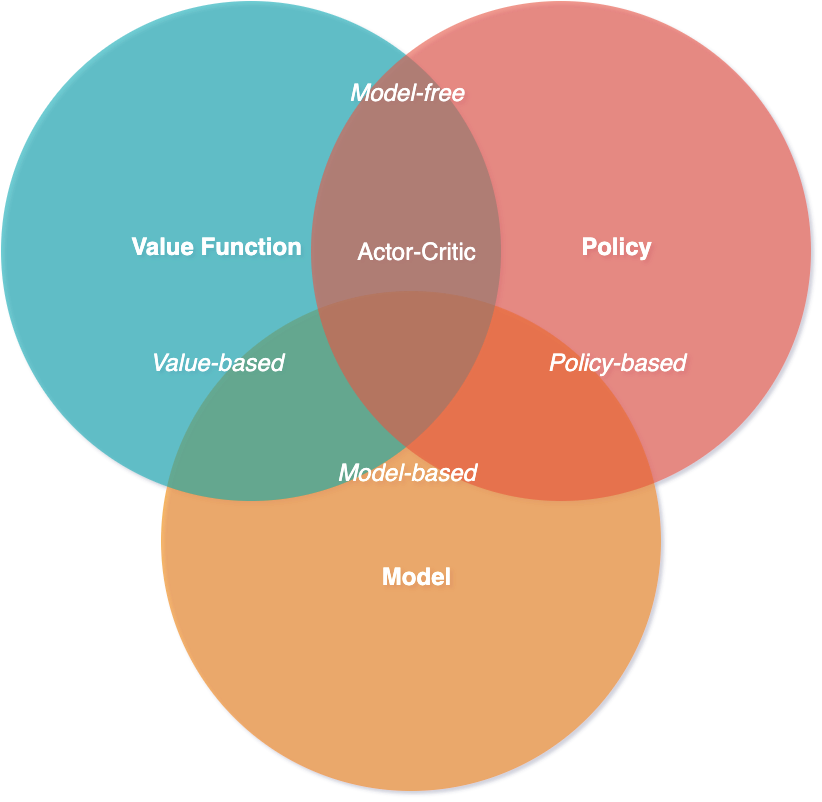
\includegraphics[width=0.65\textwidth]{silver-venn}
\end{figure}


\chapter{Q-learning and Deep Q-networks}
\section{Q-learning and Q-networks}

Q-learning \cite{Watkins1992} appeared in 1992 and is considered one of the early breakthroughs of RL \cite{rlai}.
It is a simple algorithm allowing an agent to learn an optimal policy in an unknown environment.

Q-learning is part of \textbf{temporal difference (TD)} learning.
TD is a class of solution methods in RL that is part of the model-free subset \cite{rlai}.
An advantage of TD learning can learn from incomplete episodes \cite{long-peak-rl}.

\subsection{Q-learning and the Q function}
In a Q-learning problem, the focus of our optimization is explicitly on actions, depending on the state they are taken in.
What we defined in \ref{rl:value-func} is a state-value function, as it maps each state to a value representing its desirability.
The Q function in Q-learning, in contrast, is an \emph{action-value function}.

An action-value function \(Q(s, a)\) (for ``quality'') takes a \emph{state-action pair} as input (not just a state).
Its value is the expected return of taking action \(a\) in state \(s\), then continuing to act based on the current policy.
This value can actually be decomposed into two parts: immediate reward \(r\) given by state \(s\), and the value of the successor state \({s}'\) \cite{silver-lectures}.
This idea is captured in the Bellman Equations, which we will omit here for brevity, but can be found in \cite{rlai, silver-lectures}.

A Q-learning agent chooses actions greedily based on their Q-values.
An optimal Q-function, denoted by  \(Q^{\star}(s, a)\), corresponds to an optimal policy (optimal behaviour for the agent).
Through the iterative process of Q-learning, our \(Q\) eventually converges to \(Q^{\star}\).

Q-learning is useful in problems with a finite number of states and a finite set of possible actions.
In the most trivial examples, the Q function can be represented as a table, memorizing state and action.

\subsection{Q-networks}

Using a dictionary (data structure) to map state-action pairs to their values breaks down quickly in practice.
Instead, we need a more powerful model to store and update our Q-function.
A \textbf{neural network} can fill in the role of the function approximator.
This solves the data efficiency problem of Q-learning \cite{long-peak-rl}.
We call this a \textbf{Q-network}, or \textbf{deep Q-network}, denoting it is multi-layered.
``The Q-network can be a multi-layer dense neural network, a convolutional network, or a recurrent network, depending on the problem'' \cite{long-peak-rl}.

\section{Atari DQN}

Unfortunately, using a neural network to approximate the Q-function introduces additional complexity to the problem.
Whereas classical Q-learning is shown to be stable and manages to converge to the optimal values under easily-met conditions \cite{atari-dqn},
taking the Q-network approach may introduce \textbf{instability} and \textbf{divergence} \cite{long-peak-rl}.

\textbf{Atari DQN} \cite{atari-dqn} tackles those issues by introducing two key concepts: experience replay and a target network. In the upcoming section, we explain these crucial improvements.

\subsection{Experience Replay}

Experience replay refers to keeping a replay queue in memory and sampling episodes at random from this queue \cite{atari-dqn}.

Firstly, experience replay boosts the sample efficiency of Q-learning. Q-learning is an online learning algorithm: given a sample, it will consume it to adjust its values.
This immediate discarding can lead to forgetting, thus producing suboptimal behaviour.
Storing samples overcomes this problem.

Secondly, random sampling is important due to the nature of the data.
To explain why replay grants a significant advantage, let us consider a more popular use-case for neural networks: classification problems.
In supervised learning, a correct training set contains samples that are \emph{uniformly distribuited}.
Our problem differs significanlty in definition: our input data is sequential.
(Game states obtained from the Atari emulator are highly correlated.)
Using highly correlated data to train our Q-network can easily lead to overfitting \cite{jaromiru-dqn}.
Thus, it is better to sample episodes at random instead of training in an ordered sequence.

In DQN, the capacity of the replay memory is limited, as specified by a hyperparameter \(N\). When the memory is full, it discards the oldest sample.

\subsection{Target Network}

In Q-learning, the \(Q\) function is updated based on its own values.
In a Q-network, this would translate to updating the network based on its own parameters. This can introduce instability and divergence \cite{jaromiru-dqn}.

The idea of a target network is simple in principle:
every \(t\) time-steps, we take a snapshot of the main network's parameters and use them to create a \textbf{target network}.
The target network is \emph{frozen} \cite{long-peak-rl} until the next snapshot.
Between snapshots, \(Q\) is optimized based on values of the target.
This significanlty reduces oscillations, increasing stability of learning \cite{atari-dqn}.

\section{Rainbow DQN: The state-of-the-art}
% * show the graph in the rainbow paper
% * a series of improvements: list them all
% * take 2 subsections to explain 2 easier improvements?
% * mention Sonic the Hedgehog(tm) benchmark and cite it

\chapter{Application in Grid Worlds and 2D Games}
\section{In Atari DQN}

\section{In Grid-based Games}

\chapter{Conclusion}
The transfer of knowledge from deep learning to the classical methods in RL is revolutionizing the field.
Q-learning has evolved a long way since its inception in 1992.
Off-policy TD-control methods have shown a promising evolution, shifting from inefficient tabular representations to neural networks and other powerful ML models.

At the same time, despite being marked by the success of AlphaGo and its variants, RL agents are not yet prepared to handle real-world problems.

The study of autonomously learning RL agents in games has also been challenging.
As we have seen with DQN and its successors, its greatest weakness remains sample efficiency -- agents need to train for millions of steps before they demonstrate any significant amount of ability.
And even then -- as pay closer attention to generalization in deep RL -- we find that most methods fail to manifest the ability to generalize, outside of very simple strategies (such as Breakout or Pong).

With this in mind, the future looks bright, with a new recently released paper from DeepMind -- \emph{Agent57} (2020) \cite{agent57-paper}.
The latest research trends seem to be using mixed approaches: DQN and policy optimization algorithms, in an attempt to break the barriers set by their predecessors.
Agent57 has managed to break every record on the Atari benchmark and has obtained scores above the human baseline on each of the 57 games in the set.


\bibliography{references}

\end{document}